\documentclass[12pt,a4paper]{report}
\usepackage[hmargin=3cm,vmargin=3cm]{geometry}
\usepackage{graphicx}
\usepackage{caption}
\usepackage{gensymb}
\usepackage{array}
\usepackage{ragged2e}
\usepackage{listings}
\graphicspath{Images}
\usepackage{hyperref}


\begin{document}

\begin{figure}
	\centering
	
\includegraphics[width = 0.3\textwidth]{iit}
	\hspace{1cm}
	
\includegraphics[width = 0.4\textwidth]{fossee-logo}
\end{figure}

\title
	{\textbf
			{\textbf
				{Summer Fellowship Report}}
				\vspace{5mm} 
				\\\small On 
				\\\vspace{5mm} 
				\textbf
				{\large PROJECT RECYCLE : AN ANALYSIS OF SOLID WASTE MANAGEMENT SYSTEM IN THIRUVANANTHAPURAM MUNICIPAL CORPORATION}
				\vspace{5mm} 
				\\\vspace{5mm}
				\small Submitted by
				\\\vspace{5mm}  
				\large 
				\textbf
					{TEAM BITPLEASE :}
					\small AJAY RAGH, AKHIL M, ASHIQ MEHMOOD, ASWIN S, MIDHUN C KACHAPILLY, RAAMESH BHARDWAJ	
					\\ \vspace{5mm}
				\small Under the guidance of \\ \vspace{5mm}
				\large 
				\textbf{Prof.Kannan M. Moudgalya} 
				\vspace{1mm}\\ Chemical Engineering Department  \vspace{1mm} \\IIT Bombay
}
\vspace{1cm}


\maketitle


\newpage
\title{\textbf{\textbf{\LARGE 
\begin{flushleft}
\textbf{Acknowledgment}
\end{flushleft}
}}}
\begin{justify}
	
We are fortunate to have an amazing mentor, Mr. Venugopal Pai, who has helped us push our limits and guide us whenever we are stuck. Without his tremendous support, we wouldn’t have gotten this far. Therefore, our first and foremost gratitude goes to him. Next, our sincere gratitude and appreciation go to Dr. Kannan M Moudgalya, Professor at the Department of Chemical Engineering, IIT Bombay and the department of FOSSEE for providing us with this wonderful opportunity. Special mention to Ms. Smita Wangikar of team FOSSEE at IIT-B, who has guided us through the procedures of this fellowship program.
\vspace{5mm}
\\We would have never known about this fellowship program if it were not for Mr. Vishnu Easwaran, Research Associate at IIT-B and a mentor to all of us. Special thanks to Mr. Akhil S G and all the members of Sahridaya for their constant support and encouragement. Ms. Deepthi J Patric of ICFOSS, TVM, who helped us with the software QGIS.
\vspace{5mm}
\\This was a data analysis project, which requires the collection of data, which would not have been possible without the help of people at the Thiruvananthapuram Municipal Corporation (TMC) office. Our sincere gratitude goes to the Mayor, Mr. V K Prasanth and the Collector, Dr. K Vasuki IAS. Mr. Anoop Roy, the Health Inspector at TMC office and Mr. Nikhilesh Paliath of Thanal who had enlightened us with the workings of the waste management system. The HI’s of other circles who have provided us with the required data. The technicians who work at the Aerobic bin unit facilities for their excellent cooperation.
\end{justify}

\tableofcontents

\chapter{\textbf{Introduction}}
\begin{justify}
Solid waste management and disposal are one of the most emerging challenges of the modern world, especially in economically developing countries due to their growing populations, lifestyle change, rising community living standards and increasing waste generation rates with the consequent increase in land requirements for waste disposal and dumping. We were able to understand that the major initiatives in Thiruvananthapuram city over the last 3 years were regarding solid waste management and to turn it into a green city. The following initiatives were taken under the program to drive the change:-
\end{justify}

\vspace{5mm}

\begin{itemize}
\item Green protocol implementation
\item Decentralized Waste Management
\item Green Army - a platform where individuals and groups work with school students to educate them about  segregated waste management and other sustainable living practices in an urban environment
\item Waste management awareness festivals
\item Zero waste ward initiative
\end{itemize}

\vspace{5mm}

\begin{justify}
From our discussions, we identified a need for an impact analysis of the initiatives and generate performance models that could be used to implement the above initiatives in other districts in Kerala. Multiple innovative solid waste management technologies were also implemented along with the drive-in different parts of Trivandrum, we had identified that the impact analysis and optimization of the same were other requirements.
In our project, we wish to include:-
\end{justify}

\begin{itemize}
\item Data collection from various organisations, government bodies, health inspectors and Green Army volunteers across the city.
\item Engaging with recognised organisations in the field of solid waste management to identify Key Performance Indicators.
\item To do an analysis of existing inflow and outflow, and assist government agencies in identifying gaps and engage in capacity building activities.
\item Identifying and generating models to optimize the new technologies that were implemented as part of the initiative.
\item Generate a template for easy implementation of the above initiatives in other districts.
\end{itemize}



\chapter{\textbf{About the Area Under Study}}

\section{Thiruvananthapuram City - An Overview}
\begin{justify}
	Thiruvananthapuram is a coastal city located at 8$^\circ$ 30' 30.77" N latitude and 76$^\circ$ 57' 9.37" E longitude along the south-western corner of India. The City is spread over an area of 214.86 km sq. The Average population in the city is nearly 9.60 lakh (as per Census 2011). This population is distributed over 100 wards for administrative purposes. The average population density is 4,470 people per Sq. Km. The Literacy rate city is 86.75\%. The Language spoken is Malayalam. Other Languages include English,Tamil,Hindi. There are 181 Government schools in the city and about 20 Anganwadis.	
	\vspace{3mm}
\end{justify}
\begin{justify}
		\centering
		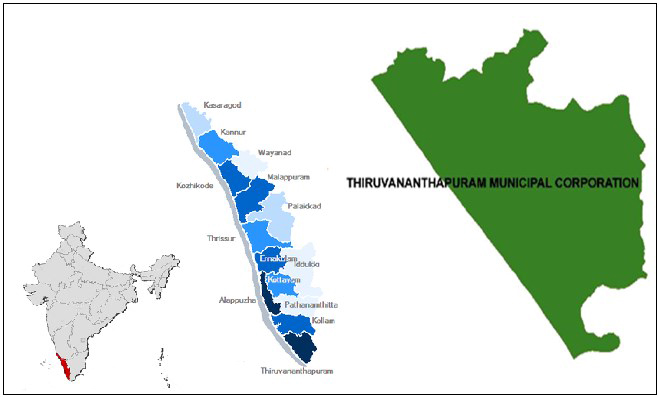
\includegraphics[width=0.75\textwidth]{ward_map_of_tvm}
\end{justify}
\vspace{5mm}
\begin{justify}
	Topographically, the city is not uniform with elevation gradually rising from sea level in the west. The city is sandwiched between the Western Ghats and the Arabian Sea. The city is built on hills by the seashore. The region can be divided into three geographical regions, the lowlands, the midlands and the highlands. The city has a coastline of 28 km long. Beach sand, sand, silt, and clay admixture (flood plain) of Holocene found in the western coastal margins and along the banks of rivers and streams. Ponmudi and Mukkunnimala are hill resorts near the city.
	The city has a tropical climate and therefore does not experience distinct seasons.In addition, nearness to the Lakshadweep Sea also modifies the climate by providing a moderate influence.The annual mean maximum and mean minimum temperature in the city are 36.2$^\circ$C and 23$^\circ$C respectively.The annual average rainfall as about 1835 mm.The rainfall is mainly received during South West Monsoon season followed by North-East Monsoon and pre-monsoon (March-May). The humidity is high and rises to about 90\% during the monsoon season.
	
	
\end{justify}	
\chapter{\textbf{Waste Management Systems}}
\begin{justify}
	The waste management system is broadly classified as centralized and decentralized. Industrialist countries such as the USA and Europe faced the problem of increasing waste production first and hence innovations and technological development of waste management strategies came from Europe and the United States. These innovations were focused mainly on the centralized waste management system. India followed suite with a focus on composting because of the large quantity of biodegradable waste in its waste stream.
\end{justify}
\section{Centralised}
\begin{justify}
	In the older central waste management system, Thiruvananthapuram Municipal Corporation (TMC) established a Municipal Solid Waste (MSW) processing plant at the nearby Vilappil Grama Panchayat (VGP), through a private agency. The estimated MSW generation in the Corporation was approximately 250 metric tonnes per day. The operator was required to establish an MSW processing plant of 300 metric tonne capacity. But the plant established by the operator was 156 metric tonnes only. Waste was to be processed through aerobic composting, i.e., conversion of biodegradable waste to soil enricher aerobically in windrows. However, the plant did not adhere to the specifications. Because of this, the conversion efficiency of the plant was reduced from 50 percent to 12 percent. This prolonged the processing period of the waste leading to ineffective utilization of the installed capacity of the plant. Due to improper and inefficient operation of the plant, the number of rejects deposited in the plant premises was about 80 percent of the MSW supplied to the plant. The anaerobic conditions caused bad odor and environmental problems and thus adverse public opinion about the workings of the plant leading to widespread conflict and protests. VGP forcibly closed the plant on 21 December 2011.
	The problems of centralized waste disposal systems are many, the waste dumping sites in and around the cities emit methane due to anaerobic digestion of organic discards. And they emit a large volume of carbon-di-oxide when these waste piles are burnt. Burning waste piles and stinking dumpsites are a common scene all over India. Centralized solid waste management systems require transportation of waste which indirectly adds to global warming through the consumption of fossil fuels.
	
\end{justify}
\section{Decentralised}
\begin{justify}
	In the case of the TMC, up until 2013, the method used was a centralized method and collected waste was mostly dumped into MCW plant at VGP mentioned above. After its shutdown,  the corporation started adopting various strategies in implementing Decentralised Waste Management. In the decentralized waste management system, waste is segregated and processed at the source. Composting is a common method used for the treatment of biodegradable waste. Non-biodegradable wastes are collected and made available for recycling processes. Thus Decentralized waste management sets a resource loop which diverts as much waste as possible from filling up landfills, which cause a nuisance to the environment and human beings.
	
\end{justify}
\section{Overflow System}
\begin{justify}
	The major problem with households in the TMC area is that they are densely packed, that is there is not enough free space outside the house for the waste to be used or processed. Building a compost requires space and nowadays with increasing population density in the urban areas it's hard for the waste processing at the source level. Thus, in Thiruvananthapuram, an Overflow method of waste management is followed, in which after segregation and management at the source level, the excess is collected by the TMC and processed.
	
	Today solid waste management is taken from a different perspective of resource use and management in the background of climate change challenge. Zero Waste is the new approach adopted by many governments across the world and a campaign is on “Zero Waste for Zero Warming” which essentially focusing on eliminating the sources of GHGs and sinking the GHGs.
	
	The Municipal Corporation of Thiruvananthapuram is trying to implement principles of a carbon-neutral city. When the city stopped its centralized solid waste management facility at Vilappilsala and launched source-level management of organic waste, it could save about Rs. one crore per year on diesel consumption for transportation of waste. This is supported further by incorporating principles of urban agriculture with decentralized waste management principles.
	
\end{justify}

%\chapter{\textbf{Solid Waste Management in Thiruvananthapuram Municipal Corporation}}
%\section{Waste Generators}
%\begin{justify}
	
%\end{justify}
%\section{Types of Solid Waste}
%\begin{justify}
%\end{justify}
%\section{Management of Biodegradable Waste}
%\begin{justify}
%\end{justify}
%\section{Management of Non-Biodegradable Waste}
%\begin{justify}
%\end{justify}

\chapter{\textbf{Date Collection Process}}
\begin{justify}
	The existing method of waste management is entrusted with the health department of Trivandrum Municipal Corporation(TMC). Initially, our team had several meetings with Health Inspectors (H.I) available in TMC office. They gave us a clear idea of the current objectives of decentralized method and existing technologies used. Also we learnt that trivandrum was divided into 25 circles and each circle was controlled under the supervision of assigned H.I.
	
	Our team went to each H.I in-charge of the Aerobin unit and/or Material Recovery Facility(MRF) of a particular ward to ask permission for accessing the data available. Further we went to each facility which was maintained by technicians working in shifts, to acquire the information regarding the waste inflow, waste processing rate and outflow. All the inflow and outflow of waste of that particular day was recorded in a ledger book. Along with this process, we used a tool called Open Data Kit (ODK) to record the information such as ward name,ward number, latitude and longitude of that facility.
	
	\vspace{5mm}
	\centering
	
	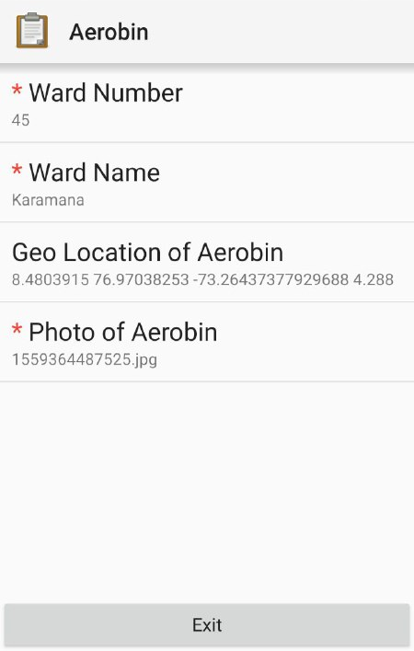
\includegraphics[width=0.4\textwidth]{odk}
	
	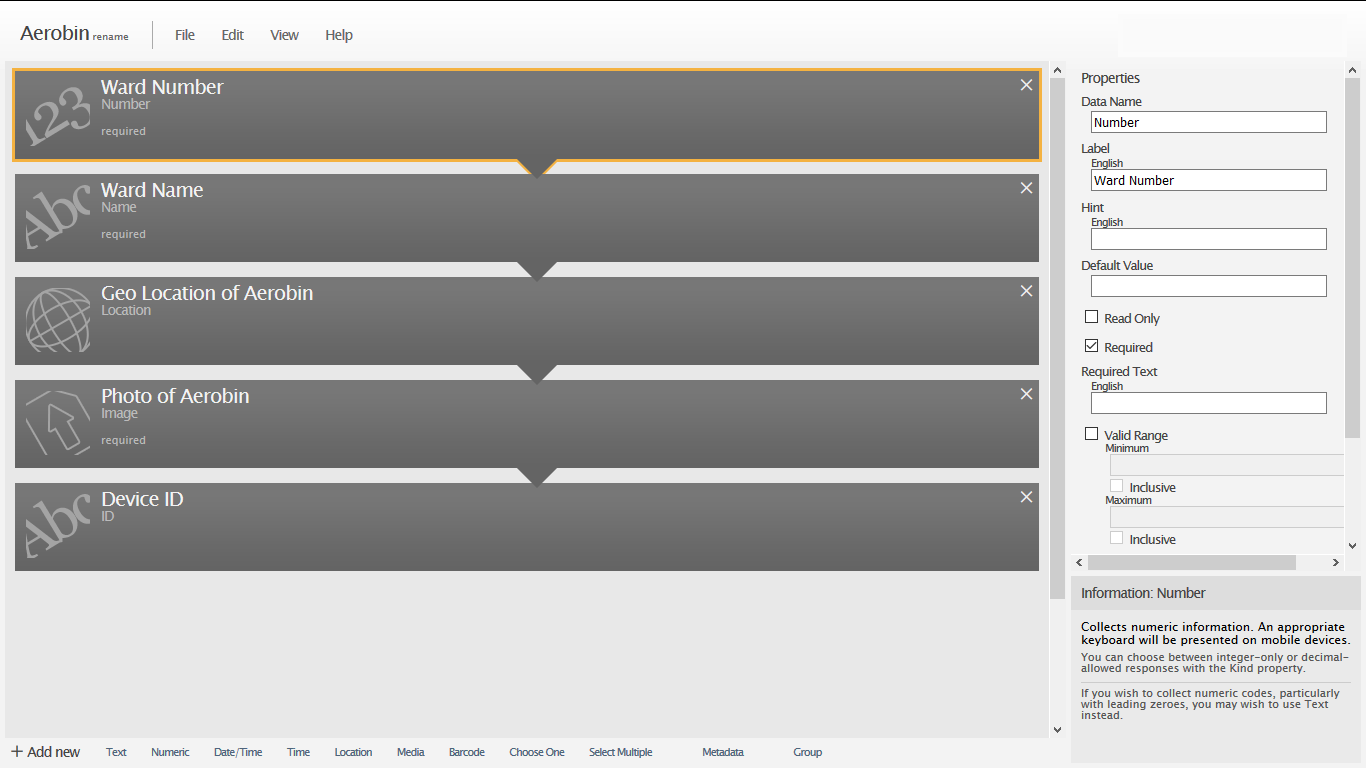
\includegraphics[width=1\textwidth]{ODKbuild}	


\end{justify}

\chapter{\textbf{Data Analysis}}
\begin{justify}
    After completing the data collection, it was sorted for further analysis purposes. Data from the ledger book was manually entered in LibreOffice Calc and then imported to Rstudio as Comma Separated Values(.CSV) files. The recorded information from ODK was then exported as.CSV files and then given to another software known as QGIS. QGIS is a free and open-source cross-platform desktop geographic information system application that supports viewing, editing, and analysis of geospatial data. It helps us to compose a map according to the information recorded from the ODK tool. It allows the person using this map to find out the nearest location of the aerobic bins.
   	Rstudio allowed us to analyze and create visuals of the CSV files with ease. Different libraries that improved the functionality for plotting interactive graphs include: 
\end{justify}
	
\begin{itemize}
\item ggplot2 - Enables creative plots. The functions such as qplot, ggplot, geomline etc.
\item plotrix - Enables creating 3D pie chart models
\item graphics - Enables creating visual graphs and analyse models with built in functions such as barplot, abline, coplot, predict etc
\end{itemize}

\begin{justify}
    Using logical programming methods in R, we analyzed the collected data and derived mathematical models to study the existing system in Thiruvananthapuram city.  Also, it was then proposed for other cities to study the feasibility of the model.
\end{justify}	

\section{Waste Inflow and Outflow over Time}
\begin{justify}
	For every ward, the capacity of aerobic is chosen according to the waste generation of that per day. In an average aerobic bin unit, there are about 10 bins each having a capacity of 1.5 Tonne. Also, the outflow from a particular facility starts only after 30-35 days from its installation period. This is the duration taken for the wet waste stored in the bin to be properly segregated and converted to compost which has a large demand in farming, gardening, etc.
	
	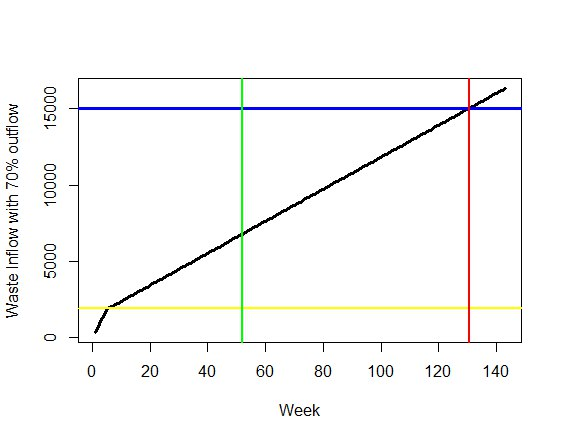
\includegraphics[width=1\textwidth]{wio}
	
	In an average aerobic bin unit, the net inflow of biowaste is about 50kg. After a month and a week, an outflow of a 70 percent rate is observed. This rate sets a balance to prevent the overflow of bin capacity and also maintain a specific amount of compost as inoculum for further stages of decomposition. 
	
	We can see a steep rise in graphical line till the week at which outflow starts, and this is represented using a yellow horizontal line. Following the 6th week, the inclination reduces and continues in a  positive direction since there is a remaining portion of 30 percent after outflow which gets added to the subsequent inflow. The green vertical line represents the week till which existing data is available. By extrapolating the graphical line, we could predict the overflow period of an average aerobic bin unit. The red vertical line shows the predicted week at which an average capacity of aerobic bin facility is less than the net waste processing rate. 
	
\end{justify}
\section{Waste Processing Capability}
\begin{justify}
	The waste processing capability of each of the wards was estimated during the project. The metric used for estimating the same was a ratio of the amount of waste processed per day in the facilities in these wards to the total amount of waste produced per day by the total population of the wards. 
	The amount of waste generated per capita per day was assumed to be around 0.4 kg(NEERI, 1996).
	The total amount of waste processed per day by the different facilities was found from the data in “Solid Waste Management-DPR” which was consolidated by the corporation of Thiruvananthapuram.
	
	\centering
	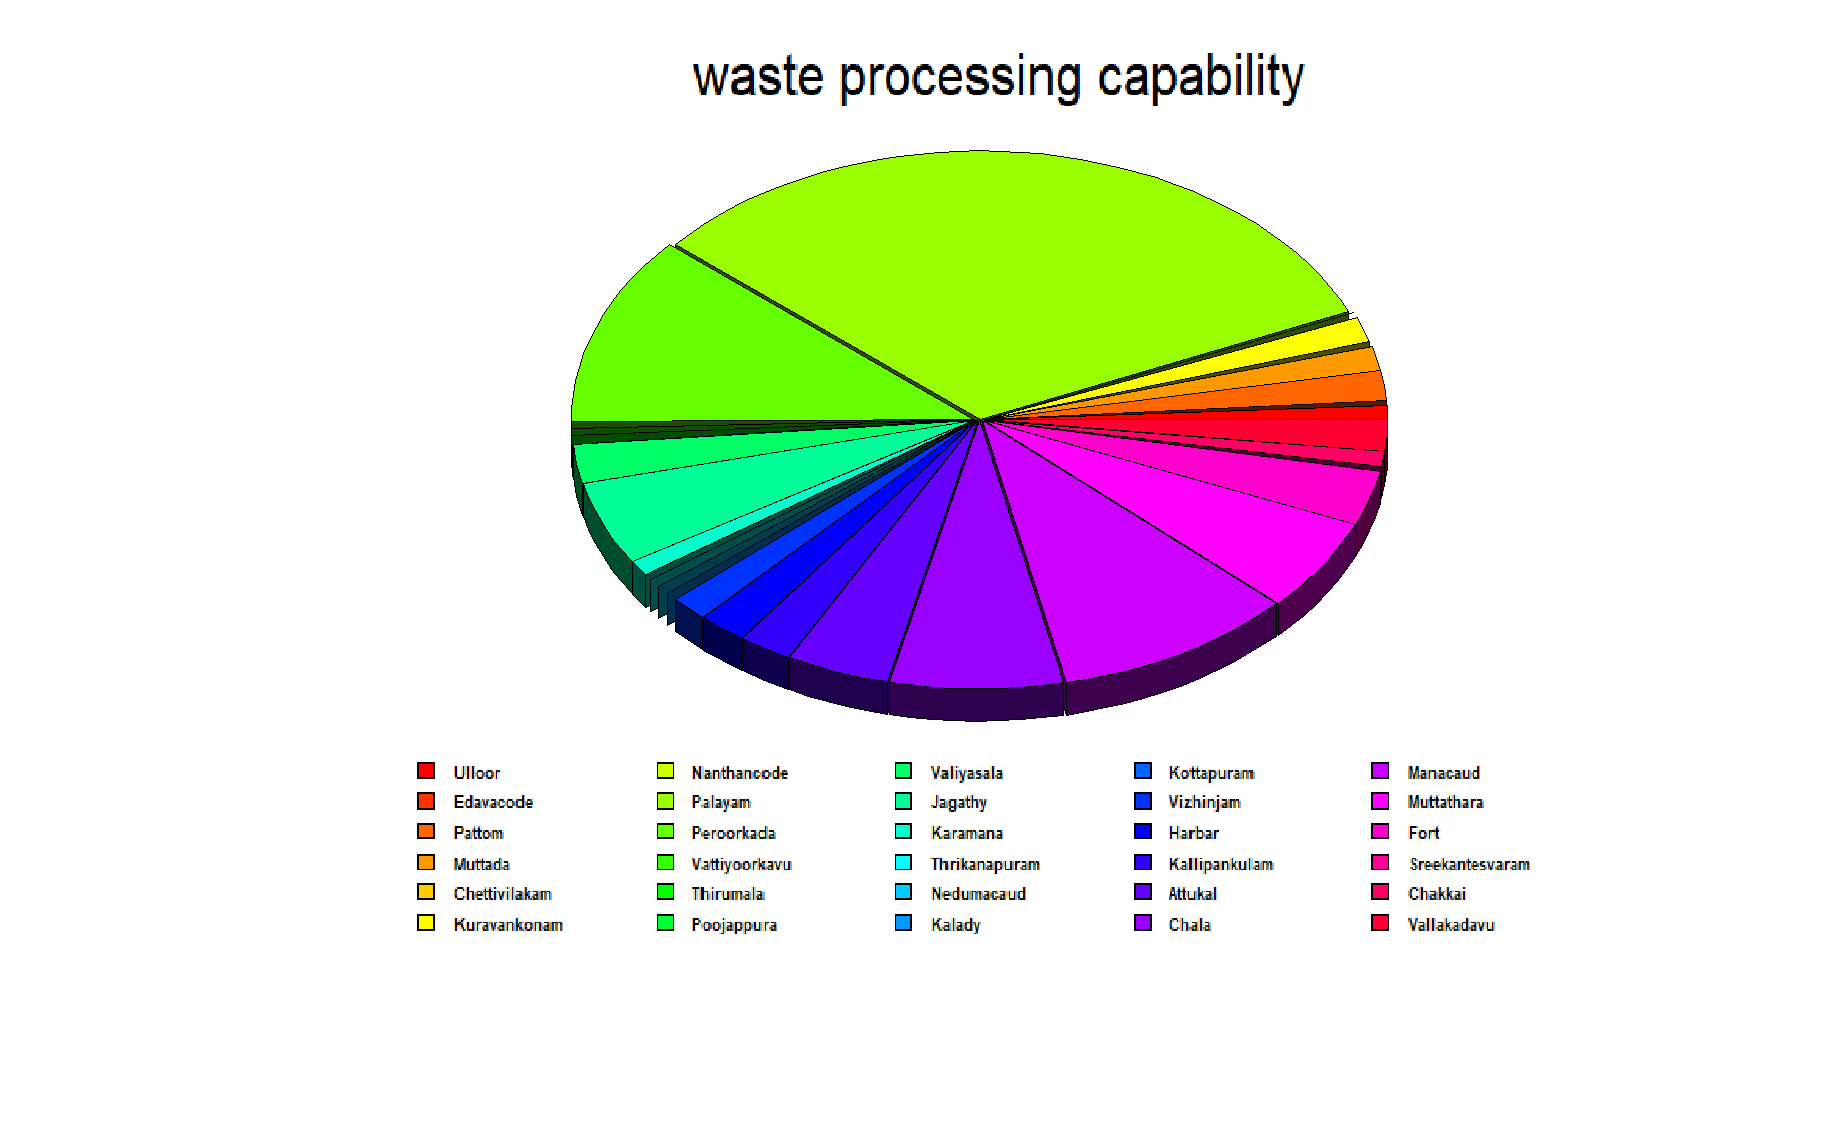
\includegraphics[width=0.75\textwidth]{wp}
	

	
\end{justify}
\section{Waste Inflow from Collected Data}
From the data collected from different facilities, the average daily inflow of waste to these facilities were calculated by summing up the total waste collected to the total number of days took to collect this amount of waste. This data was then divided into three groups of facilities with a low, medium and high inflow of waste per day. The facilities having less than 50 Kg of waste inflow per day are categorized as low inflow facilities, The facilities having waste inflow between 50-150 Kg waste inflow per day are categorized as medium inflow facilities and those having more than 150 kg waste inflow per day are taken as high inflow facilities. This data is then represented in  the form of a pie chart as shown below :

\begin{justify}
	
	\centering
	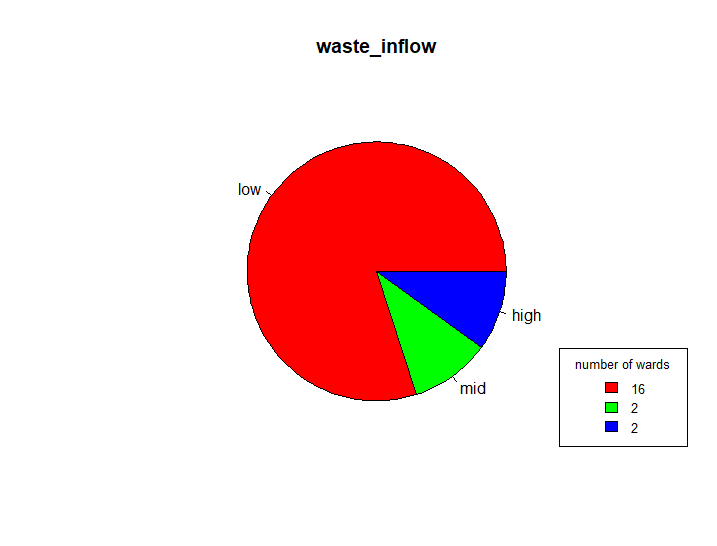
\includegraphics[width=0.75\textwidth]{wi}
\end{justify}
\begin{justify}
	From this pie chart, we can see that the vast majority of the facilities are having only a low inflow of waste per day. Only a total of 4 facilities comes under medium and high inflow facilities. This shows that for a large number of facilities are not having their capacities utilized effectively.  

\end{justify}	

\section{Waste Generation Density}
\begin{justify}
	Here, we have made a simple representation of the data regarding the waste generation and population of Wards. In the table below, the details of the Wards are given. A graphical representation is made using this data. On the abscissa, we have the population and on the ordinate, we have the waste generated per day. Each of the dots in the graph represents a Ward and the size of the dot represents the waste generated per capita per day, or as we termed it, waste generation density. The color represents the range of the waste generation density; blue being closest to the average waste generated per capita of the city, red being more and green being less than that.
	
	
	
	We can see by tracing the blue dots that the waste generated is almost proportional to the population. But as shown by the red and green dots, there are a few exceptions to this case. This is mainly due to the presence of the main market places of the city in the Wards denoted by red, and predominantly rural areas with source-level elimination of waste in the Wards denoted by green dots.
	\vspace{1cm}
	
	\centering
	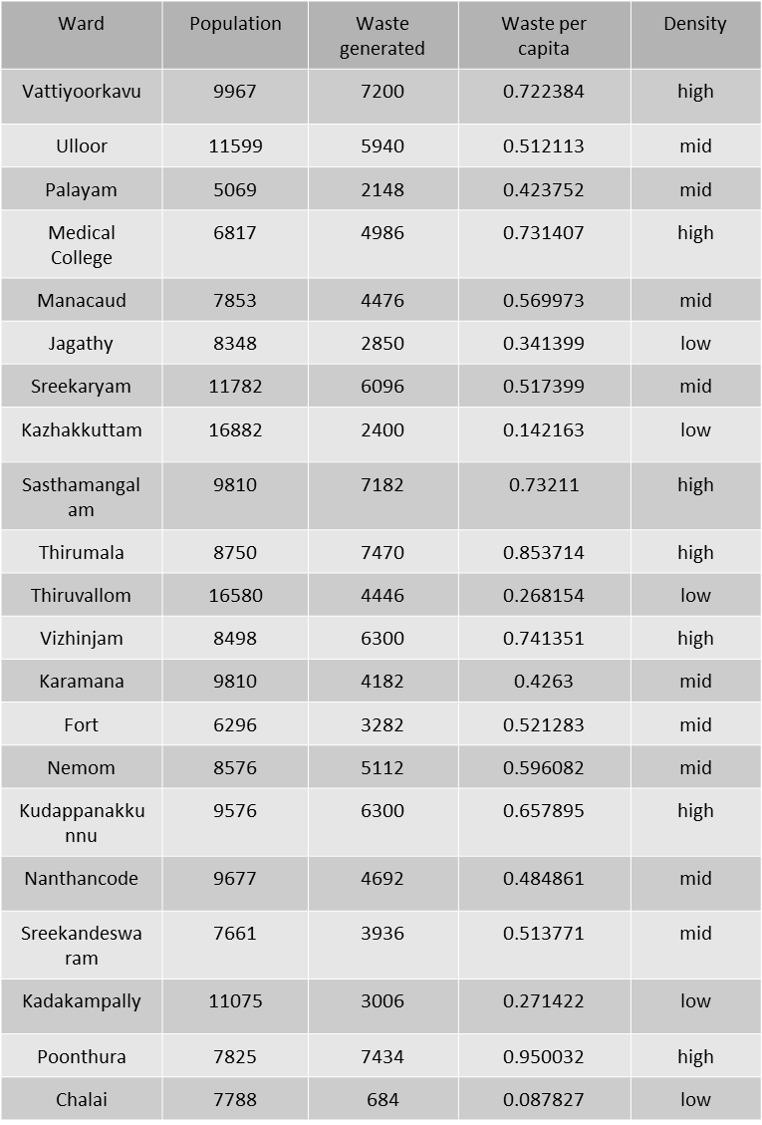
\includegraphics[width=0.85\textwidth]{table_waste_dens}
	\vspace{1cm}
	\hspace{5mm}
	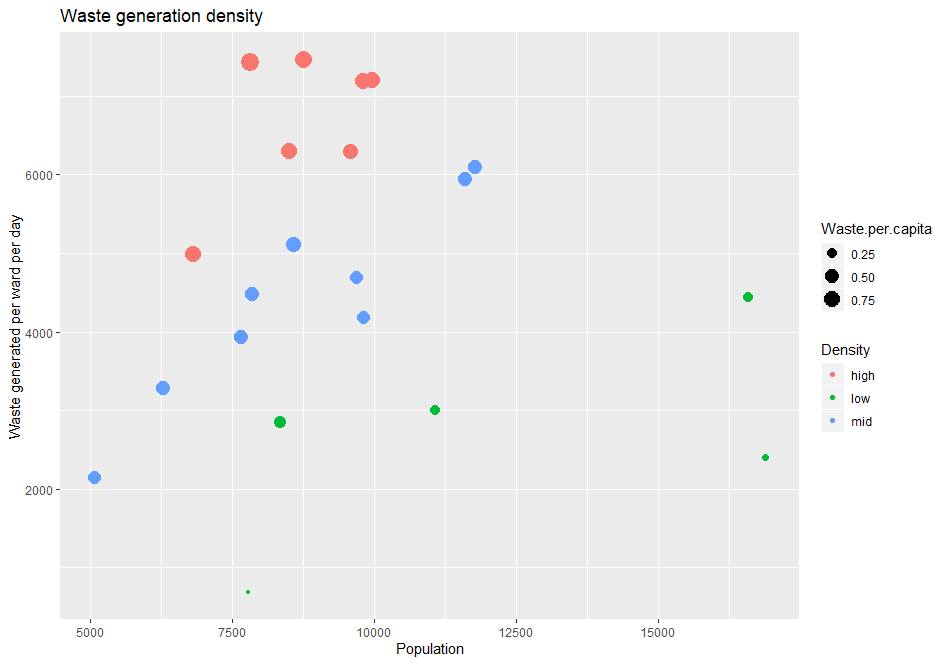
\includegraphics[width=1\textwidth]{wgd}
	
\end{justify}
\section{Working with QGIS} %To be changed
\begin{justify}
    QGIS (previously known as Quantum GIS) is a free and open-source cross-platform desktop geographic information system (GIS) application that supports viewing, editing, and analysis of geospatial data.
	The mapping of all the collected data, creation of heatmaps and plotting out the required sites of MRFs using the mathematical model all have been carried out in the open-source Geographic Information System (GIS)  software QGIS.
	The QGIS versions 3.4(Madeira) and 3.8( Zanzibar) for all the analysis purposes.
	Open Street Maps was used as the basic map layout for plotting the data. 
	
	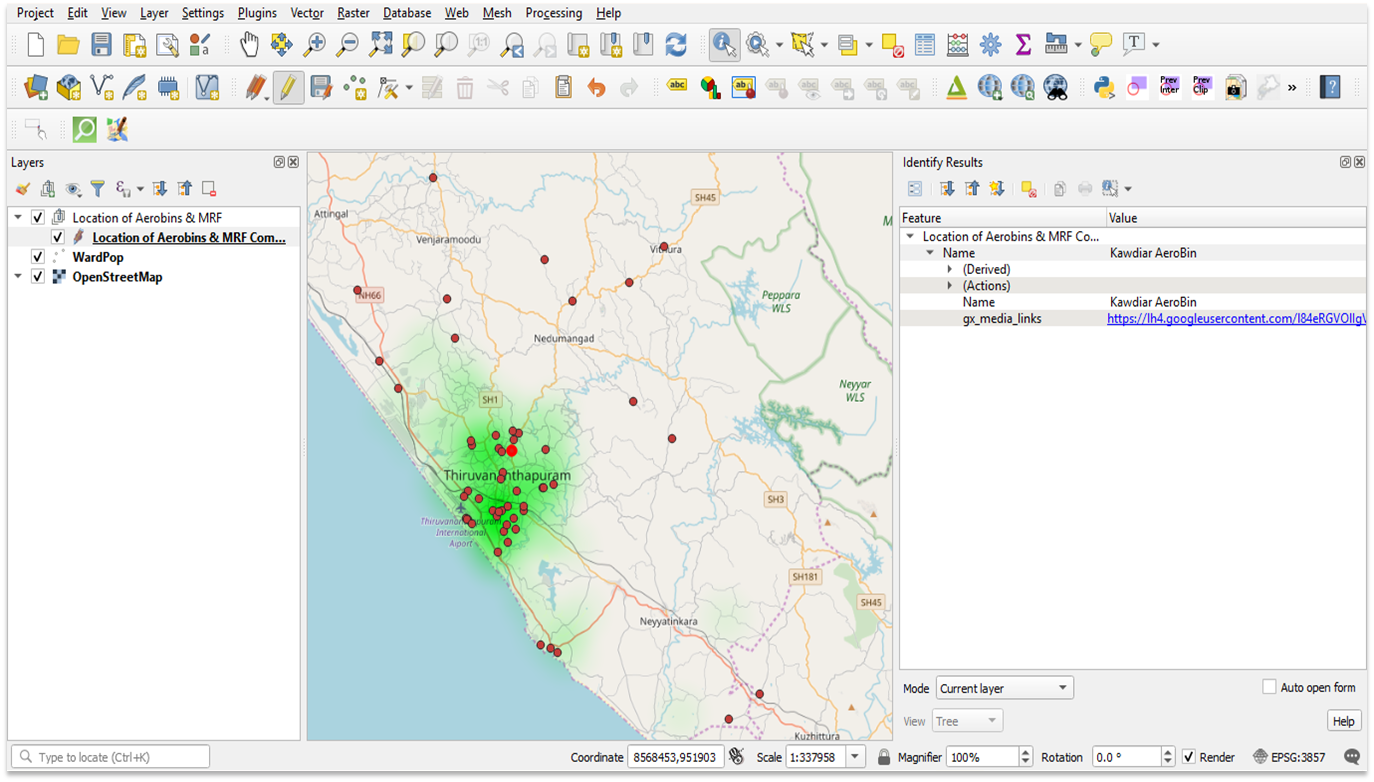
\includegraphics[width=1\textwidth]{qgis_ui}
\end{justify}
	


\chapter{\textbf{Mathematical Model}}
One of our main objectives was to generate a mathematical model for an optimum waste management system. As our scope of the study is on biodegradable solid waste, our model will be optimized only for the management of those wastes. In the current waste management system of TMC, the main way to deal with biodegradable solid waste is by using aerobic bins, the details of which have been mentioned in the earlier sections. The other ways in which the waste is discarded include source-level eliminations like pipe compost, bio compost, biogas plants, etc. which are mentioned in the section containing overflow system of waste management.
%\vspace{5mm}
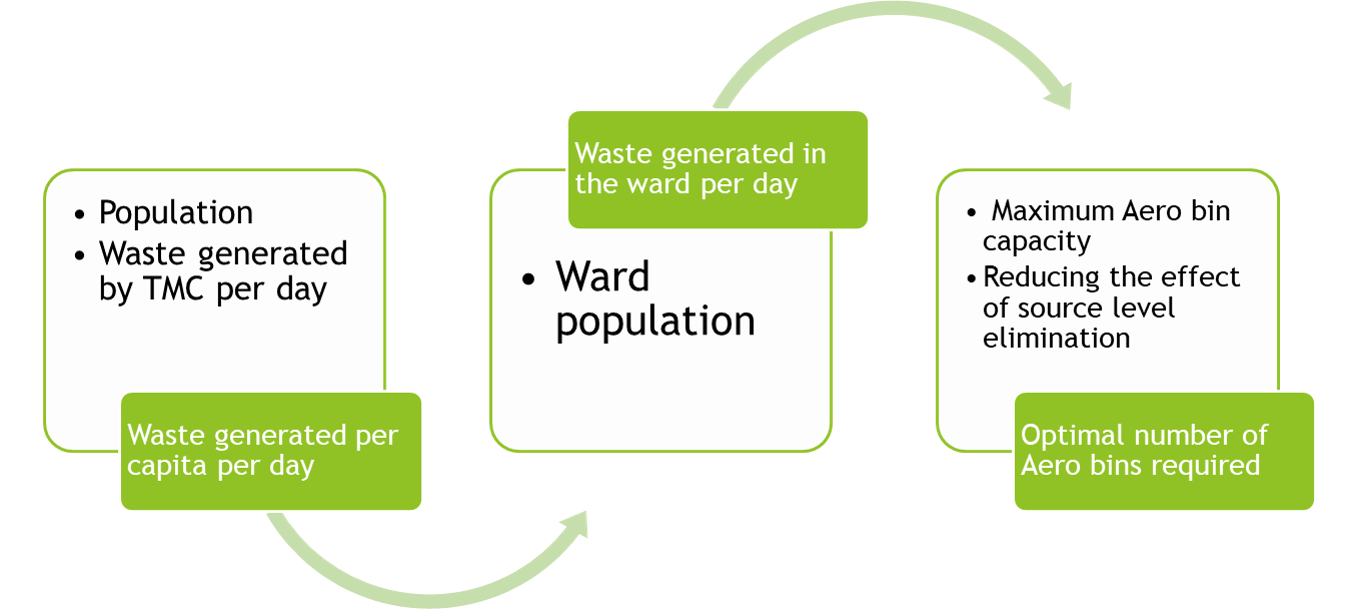
\includegraphics[width=1\textwidth]{mathmod}
Under the context mentioned above, our mathematical model would be calculating the number of aerobic bin units required and their respective locations, in each ward. For this calculation, the basic parameters used are; the population of the corporation, the total waste generated by the corporation, the population of each ward coming under the corporation, the capacity of one Aerobin unit in a day and the effect of source-level elimination of waste within that ward. For the mapping of the locations of these bin units, the parameters involved are the ward area and its boundary.

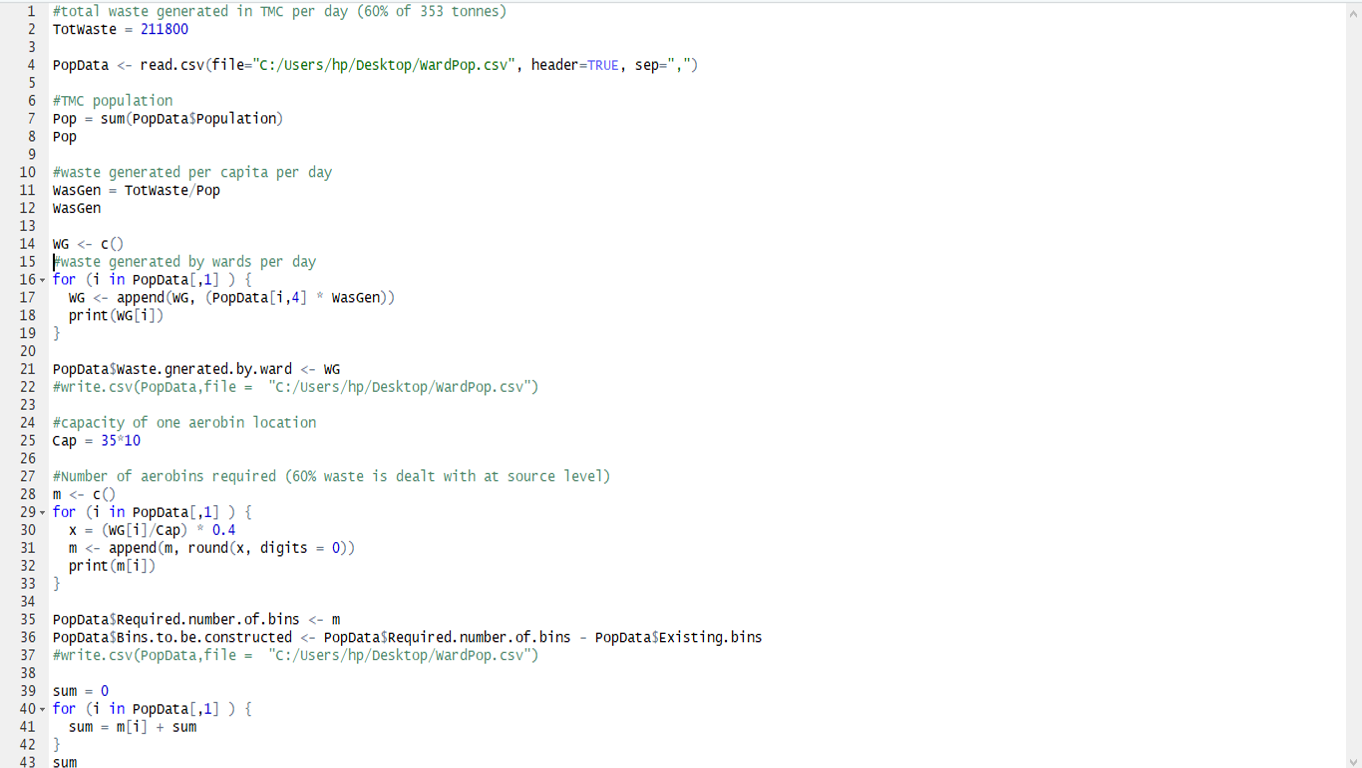
\includegraphics[width=1\textwidth]{mathmodr}

\section{Optimal Number of Bins in each Ward}
\begin{justify}
	For the first part, to calculate the required number of aerobic bin units in each ward, we take the total waste generated by the corporation in a day and divide it by its total population, we get the waste generated per capita; this value multiplied by a ward’s population would give us the waste generated by that ward in a day. The next step is to reduce the effect of the source-level elimination of waste. As mentioned in the previous sections, a portion of waste is treated at the source level itself. After reducing the effect of this factor in the waste generated by the ward, we need to divide it by the capacity of one aerobic bin unit in one day. This would give us the optimum number of Aerobin units in that particular ward.
	
	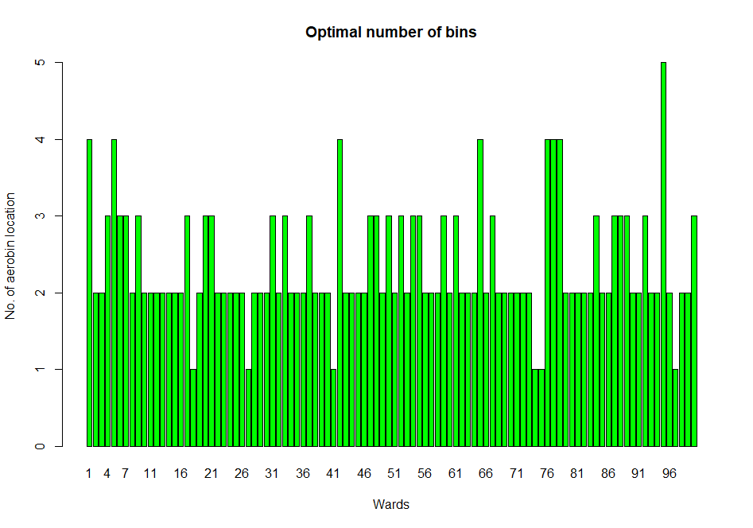
\includegraphics[width=1\textwidth]{opt}
	
	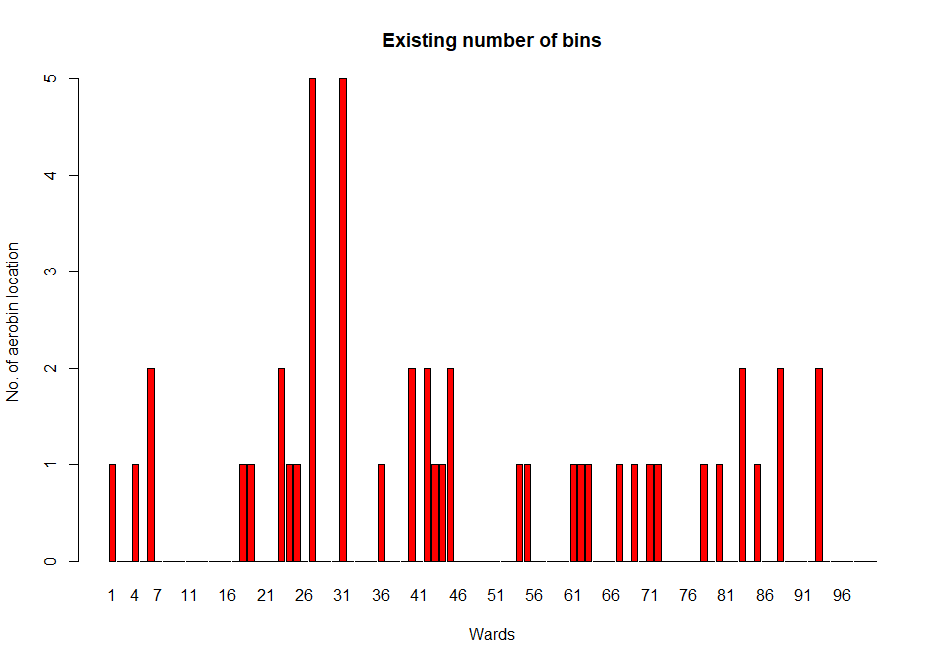
\includegraphics[width=1\textwidth]{exis}
	

	Another important point to be mentioned here is that we are calculating the optimum number of bin units. An Aerobic bin unit may contain from 4 to 10 Aerobic bins, or even more if required. What we are proposing is the desired number of locations were bin units are to be placed. The number of bins in a unit may be varied according to the waste generation of that particular ward. This would help in ease of access to waste disposal facilities for everyone in the ward.
	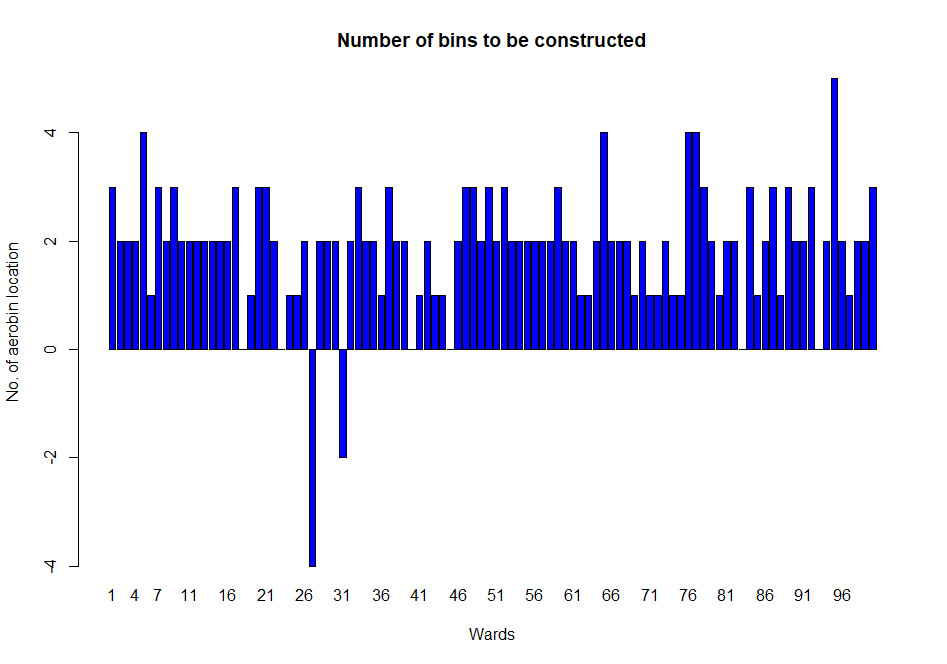
\includegraphics[width=1\textwidth]{construc}
	A common question that arises at this point is why we have used population and not area or population density for the calculation. A particular ward may contain a large area and less number of people so the waste generated may not be proportional to the area. Also, a Ward may have population density higher than the average population density of the corporation, which would result in an error while calculating the waste generated by the ward. These are the reasons why we have avoided the area and population density and instead used the population.
	
\end{justify}
\section{Suggested Locations of Bins in each Ward}
\begin{justify}
	 A plot for the proposed location of Aerobin units in each ward was made using QGIS. As per the obtained output for the collected data we were able to calculate the number of Aerobin sites required in each ward area so that it is easily accessible to all the population in the ward and also the waste distribution to be even in each site. Thus mapping out the result in Map for the whole TMC area is shown on the left which provides general insight on the number of bins to be constructed and on the right, it shows a zoomed view of a single ward which is marked in red. The division of the Ward and placement of Aerobin is in such a way that the Aerobin sites are accessible to the population in an easy way. Area divided is based on the least distance to the Bin. The green area shows a possible region of placement of an Aerobic bin site.
	 
	 \centering
	 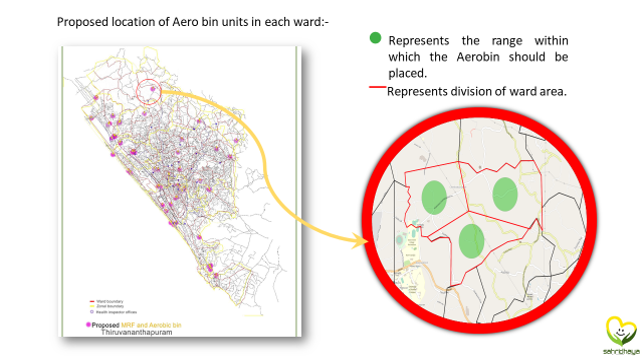
\includegraphics[width=1\textwidth]{bin_loc}
\end{justify}

\chapter{\textbf{Inference}}
\begin{itemize}
	\item From the study we conducted on TMC’s waste management system, we were able to analyze the inflow and outflow of waste.
	\item We also generated a mathematical model of TMCs Waste Management Systems and Applied it to two other districts.
	\item Although we wanted to analyze the existing system, by comparing it with the old system of centralized waste management, we couldn’t do so due to authoritative issues in obtaining the old data.
\end{itemize}






\newpage
\title{\textbf{\textbf{\LARGE 
\begin{flushleft}
\textbf{Reference}
\end{flushleft}
}}}
\begin{itemize}
\item \href{https://www.researchgate.net/publication/260230170_MUNICIPAL_SOLID_WASTE_MANAGEMENT_IN_INDIA_A_REVIEW_AND_SOME_NEW_RESULTS}{MUNICIPAL SOLID WASTE MANAGEMENT IN INDIA : A REVIEW AND SOME NEW RESULTS} 
\item \href{https://www.cag.org.in/blogs/solid-waste-management-dummies}{Solid waste management}
\item \href{https://www.downtoearth.org.in/blog/waste/india-s-challenges-in-waste-management-56753}{Report by DownToEarth magazine}
\item \href{https://www.cag.org.in/database/centralised-and-decentralised-waste-management}{Centralized and Decentralized waste Management }
\item \href{http://www.corporationoftrivandrum.in/sites/default/files/Rating\%20report-TVM.pdf}{TMC Report}
\item \href{http://thanal.co.in/uploads/resource/document/standard-operating-procedure-of-community-aerobic-composting-bins-thumburmoozhi-model-44732514.pdf}{Thanal : Operation of aerobic bins}
\item \href{http://www.kerala.climatemps.com/}{Rainfall pattern in TMC}
\end{itemize}
\end{document}


